\documentclass[twoside]{article}

\usepackage[spanish]{babel}
\usepackage[utf8]{inputenc}
\usepackage{graphicx}
\usepackage{geometry}
\usepackage{fancyhdr}
\usepackage{afterpage}
\graphicspath{ {img/} }



%FOOTER & HEADER
\pagestyle{fancy}
\fancyfoot{}
\fancyhead{}
\renewcommand{\headrulewidth}{0pt}
\fancyfoot[RO, LE] {\thepage}
\renewcommand{\baselinestretch}{1.2} 
\geometry{a4paper,
 	total={150mm,230mm},
 	left=35mm,
 	top=30mm,
 }
 

\title{Numinum SA}

\author{Gaizka Virumbrales \& Rubén Sánchez}

\date{\today}

\begin{document}
\maketitle
\begin{figure}[ht!]
	
\includegraphics[width=100mm]{logo.png}
	\centering
\end{figure}
\thispagestyle{empty}
\newpage
\newpage
\null
\thispagestyle{empty}
\newpage

%%%%%%%%%%%%%%%%%%%%%%%

\pagenumbering{roman}

\begin{abstract}
La empresa Numinum quiere implementar un SGC y ha pedido al departamento de administración, junto al de TI un plan de implementación para este tipo de sistema.
\end{abstract}


%\renewcommand{\contentsname}{Tabla de contenido}
\setcounter{tocdepth}{2}
\tableofcontents
\newpage
\pagenumbering{arabic}
\setcounter{page}{1}
\section{Visión, misión y estrategia}

En esta sección se definen la visión, misión y estrategia de la empresa.

\subsection{Visión}
\label{sec:vision}

Ser la empresa reconocida como líder en la venta y producción de electrodomésticos por parte de sus clientes y empleados siguiendo una filosofía de respeto hacia el medio ambiente y de compromiso social.
\\
\\

\subsection{Misión}
\label{sec:mision}

Contribuir al consumo de energías renovables fabricando electrodomésticos de calidad, duraderos y respetuosos con el medio ambiente que cumplan los estándares de eficiencia energética y contribuir también la igualdad dejando de lado los estándares de la sociedad y aspirando a conseguir unas técnicas de contratación basadas en factores externos al sexo, raza, religión, nacionalidad, etc. Por último, gestionar los datos de forma que creen valor para la compañía como para sus empleados.
%
\\
\\

\subsection{Estrategia}

El objetivo de Numinum es posicionarse como líder nacional en la venta y producción de electrodomésticos y, además, ser una empresa respetuosa con el medio ambiente y ser un activo en la lucha por la igualdad social.

En Numinum trabajamos para alcanzar el liderazgo y la confianza de los diferentes estamentos sociales ofreciendo una amplia gama de productos capaz de satisfacer las necesidades de cada uno de estos estamentos.

Por lo mismo, la compañía está invirtiendo para garantizar la sustenibilidad financiera y ambiental de sus acciones y operaciones en el largo plazo, específicamente en: Capacidad, tecnologías, habilidades, personas, marcas, investigación y desarrollo.

Nuestro objetivo es satisfacer las necesidades actuales y conseguir que la mujer tome un papel más importante en las generaciones futuras y que gente con menos poder adquisitivo sea capaz de optar a unos electrodomésticos de calidad y respetuosos con el medio ambiente.
\newpage

%-----------------------------

\section{Iniciativas de GC}
En este apartado hablaremos sobre las iniciativas que hemos optado implantar, teniendo en cuenta la matriz DAFO de nuestra organización.
\subsection{Matriz DAFO}

\begin{table}[ht!]
	\centering
	\begin{tabular}{ p{6cm} | p{6cm} }
		\textbf{Fortalezas} & \textbf{Debilidades}\\
		- Servir a diferentes estamentos de la sociedad & - No contamos el dinero suficiente para crear y mantener fábricas respetuosas \\
		- Gran popularidad a nivel nacional & - El alto coste de fabricación  \\
		- Siete nuevos productos innovadores & \\
		- Nueve calificaciones ISO & \\
		- Sistemas de toma decisiones & \\
		- Alto uso de Wikis y blogs de GC & \\\hline\\
		\textbf{Oportunidades} & \textbf{Amenazas} \\
		- Subvención por respeto al Medio Ambiente & - Cierre de una sucursal o de toda la empresa por la tendencia actual\\
		- Subvención de colaboración con universidades & \\
		- Investigación de 'la casa inteligente' & \\
		- Capacidad de dar empleo a nuevos investigadores a bajo coste gracias a los estudiantes universitarios 
	\end{tabular}
\end{table}


\subsection{Páginas amarillas}
\label{sec:pAmarilla}
\textit{Elaborar unas páginas amarillas generales con el conocimiento tácito de los empleados de cada departamento y las diferentes sedes.}

\begin{figure}[ht!]
	\includegraphics[width=130mm]{EntityRelation.png}
	\caption{Entidad relación de la BD de las páginas amarillas.}
	\label{fig:entiy relation}
\end{figure}

\textbf{Justificación}: La elaboración de unas páginas amarillas permitiría a la empresa acceder a los conocimientos tácitos de sus empleados con más velocidad y eficacia.

\textbf{Descripción del proceso}: [Anexo] Proceso Paginas Amarillas

\subsection{Entrevistas a personas}
\label{sec:entrevistas}
\textit{Elegir un encargado por cada país para que actualice una DB con las normas referentes al medio ambiente en ese país, el proceso seguido para adaptarse a esa norma y que haga llegar los cambios al resto de la empresa.}
\\

\textbf{Justificación}: Realizar entrevistas a personas nos permitiría dar con la persona más .

\textbf{Descripción del proceso}: [Anexo] Proceso Entrevistas

\subsubsection{Entrevista semiestructurada}
\textit{Tema: Gestión de la normativa de una planta}\\\\
Hola [\textit{Nombre}], veo que actualmente trabajas en el dpto. de [\textit{dpto}], ¿está usted contento con su trabajo?

\begin{itemize}
	\item ¿Estaría dispuesto a asumir responsabilidades extra?
	\item ¿Se considera una persona consciente de lo que pasa a su alrededor?
	\item ¿Sería capaz de contradecir a un cargo superior basándose en una norma establecida?
	\item[\textbf{Entrega}] Le da un texto (un decreto) y tiene que extraer las normas y nuevas leyes que están implícitas en el.
	\item He visto en su CV que tiene conocimientos de SQL, nosotros trabajamos con PLSQL, ¿cree que sería capaz de aprender el lenguaje?
	\item ¿Conoce los procesos básicos de la fábrica?
	\item ¿Cree que sería capaz de modificarlos eficientemente según las normas de medio ambiente?
	\item ¿Tienes familia?
	\begin{itemize}		
		\item[\textbf{Si}] ¿Crees que la familia y el trabajo son aspectos separados de tu vida?
		\item ¿En caso de tener que ir a trabajar a una planta al extranjero, te llevarías a tu familia?
		\item[\textbf{No}] ¿Tienes pensado en tener familia a corto/medio plazo?
		\item ¿Estarías dispuesto a llevar un seguimiento de los cambios en las leyes para poder actualizar las normas de la empresa?
	\end{itemize}
\end{itemize}
Un placer haber tenido esta entrevista con ud ordenaremos las ideas que hemos extraído en un documento y se las enviaremos para verificar que hemos entendido bien todos los puntos. El proceso de selección todavía no ha terminado, en cuanto llegue a su fin le llamaremos con el resultado.

\subsubsection{Entrevista estructurada}
\textit{Tema: Gestión de la normativa de una planta}\\\\
Hola [\textit{Nombre}], es un placer tenerle aquí otra vez.

\begin{itemize}
		\item ¿Estaría dispuesto a trabajar en una planta extranjera?
		\begin{itemize}
			\item[\textbf{Si}] Seguiremos la entrevista en el idioma que predomine en la planta en la que tenemos pensado enviarle.
			\item[\textbf{No}] Seguiremos la entrevista en castellano si hay alguna fabrica que necesite de estos servicios y que su idioma predominante sea el castellano.
		\end{itemize}
	\item ¿Conoces los procesos básicos de la fabrica?
	\begin{itemize}
		\item[a)] Proceso 1
		\item[b)] Proceso 2
		\item[c)] Proceso 3
	\end{itemize}
	
	\item ¿Cual dirías que es el mas conflictivo en cuanto a ley del gobierno Taiwanes publicada en el decreto de medio ambiente TW-74/6.3? (Un ejemplo de pregunta por si el puesto fuera para Taiwan)
	\item Demuestra mediante la creación de un modulo  [\textit{Tipo de modulo}] que sabes utilizar el lenguaje PLSQL.

\end{itemize}


%%%%%%%%%%%%%%%%%%%%%%%%%%%%%%%%%%%%%%%%%%%%%%%%%%%%%%%%%%%%%%%%%
\newpage

\section{Identificación de conocimientos}

\subsection{Auditoría de conocimiento}

En Numinum contamos con 6300 trabajadores en 9 fabricas y 13 oficinas afiliadas repartidas por 10 países.\par
Estos trabajadores están repartidos en 8 divisiones corporativas que comparten todas la visión, misión y estrategia de la empresa.
Por encima de estos departamentos esta el Director General, que es elegido por una Asamblea Permanente de 10 personas, que a su vez es elegida por la Asamblea General de accionistas.

\begin{figure}[ht!]
	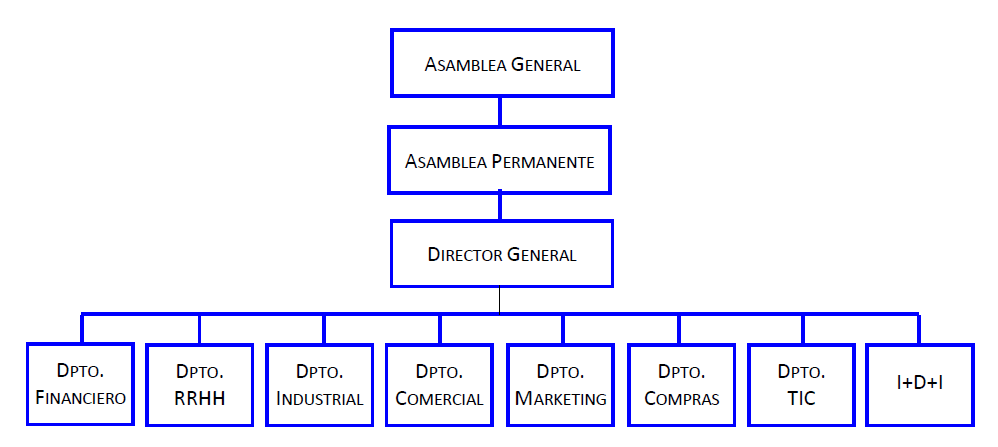
\includegraphics[width=130mm]{Organization.png}
	\caption{Organigrama de la empresa.}
	\label{fig:organization}
\end{figure}

\subsubsection{Departamento financiero}
El departamento financiero gestiona nuestros recursos económicos para la buena marcha de la empresa. Cada filial y fabrica tiene su propio control financiero, pero siempre siguiendo el plan establecido por la central.\\
Este departamento genera un balance anual a disponibilidad de los trabajadores una mayor transparencia 

\begin{figure}[ht!]
	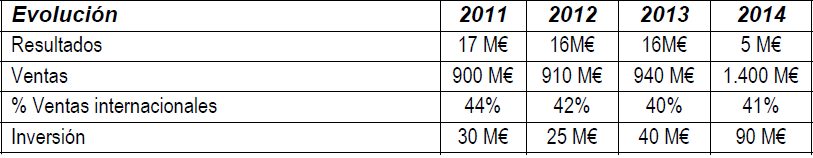
\includegraphics[width=130mm]{Finances.png}
	\caption{Tabla de evolución financiera de la empresa.}
	\label{fig:finances}
\end{figure}

%INSERTAR TABLA DE EVOLUCION
\subsubsection{Departamento de RRHH}
El departamento de recursos humanos se encarga de que los empleados reciban formación en los diferentes aspectos de la empresa, por eso el año pasado contamos con 8h de formación por empleado.
\subsubsection{Departamento industrial}
El departamento industrial cuenta con materiales de larga duración para no contribuir a la obsolescencia programada y al gasto innecesario de recursos. Las fabricas cuentan con herramientas robóticas y modernas técnicas para las cadenas de suministros.
\subsubsection{Departamento comercial}
El departamento comercial cuenta con distribuidores que llevan nuestros productos mas lejos cada día. También contamos con una Web en la empresa que permite a los cliente hacer pedidos online de nuestros productos. Por ultimo los Call Centers cuentan con personal que ha recibido formación especial para atender a todo tipo de llamadas.
\subsubsection{Departamento de marketing}
El departamento de marketing crea todos los años campañas de publicidad en la televisión, periódicos, folletos y jornadas de marketing casa por casa. También desarrolla sondeos de mercado para centrar las campañas mencionadas anteriormente a las personas que mas las necesitan.
\subsubsection{Departamento de compras}
El departamento de compras se encarga de comprar los materiales que van a ser utilizados en nuestros productos. Pedimos a nuestros proveedores que siga las normas que tiene nuestra empresa sobre calidad medioambiental. 100 de nuestros proveedores ya cuentan con, al menos, un certificado de calidad ISO 9000 o EFQM.
\subsubsection{Departamento de informática}
El departamento de informática es lo mas avanzado de nuestro sector, contamos con un amplia gamma de productos y servicios a la disposición de los trabajadores:
\begin{itemize}
	\item PDA, smartphones, Blackberries, ordenadores, portátiles, netbooks...
	\item Intranet
	\item Varios portales de Internet y webs de productos
	\item VPN
	\item Herramientas de minería de datos y ERP
	\item Equipo de informática con miembros expertos en varios campos
	\item Varios medios de comunicación
		\begin{itemize}
			\item[--] Fax
			\item[--] Videoconferencia
			\item[--] Chat
			\item[--] VozIP
			\item[--] Wikis
			\item[--] Blogs
		\end{itemize}
	\item Sistemas expertos, agentes inteligentes, DSS (Sistemas de soporte a la decisión)
	
\end{itemize}
\subsubsection{Departamento de I+D+i}
El departamento de I+D+i colabora con las universidades, centros de investigación, consorcios europeos y otras empresas ofreciéndonos así la oportunidad de crear proyectos colaborativos y que sean exitosos en el mercado.

\subsubsection{General}
La empresa en general también cuenta con un sistema propio de protección y prevención de accidentes que aumenta la seguridad en nuestras fabricas. Ademas nuestros delegados territoriales que median con los distribuidores les forman en las características de nuestros productos para que la venta al cliente final sea mucho mas fidedigna. Por ultimo todos los años celebramos una feria de "Presentación a los profesionales" donde enseñamos nuestros productos a los distribuidores y responsables de los puntos de venta.

% Relacionarlo con la captura del conocimiento %
\subsection{Lista de procesos}

\begin{itemize}
	\item Procesos estratégicos
	\begin{itemize}
		\item[--] Medición, análisis y mejora de la cadena de producción
		\item[--] Creación del plan estratégico
		\item[--] Mejorar la imagen y presencia internacional
	\end{itemize}
	\item Procesos clave
	\begin{itemize}
		\item[--] Adaptarse y adelantarse a los cambios en la normativa medioambiental de cada país I+D+i\footnote{Proceso detallado: Entrevistas a personas \ref{sec:entrevistas}}
		\item[--] Gestión optima de los almacenes de materias primas
		\item[--] Crear fabricas y electrodomésticos respetuosos con el medio ambiente
	\end{itemize}
	\item Procesos soporte
	\begin{itemize}
		\item[--] Realizar entrevistas para la elección de la persona encargada de actualizar el documento con las normativas
		\item[--] Elaborar las pruebas para superar las normas medioambientales
		\item[--] Localización y fácil utilización del conocimiento que hay en la empresa\footnote{Proceso detallado: Páginas amarillas \ref{sec:pAmarilla}}
	\end{itemize}
\end{itemize}



\newpage
\subsection{Mapa de conocimiento}

\begin{figure}[ht!]
	\includegraphics[width=150mm]{mapa.png}
	\centering
\end{figure}

\subsection{Fuentes externas de conocimiento}

Para nuestros procesos, la principal fuente de conocimiento externo es el propio gobierno y parlamento (o la institución encargada de hacer las leyes en ese país). Estar al tanto de los cambios en lo referente al medio ambiente es primordial para que nuestras fabricas cumplan con todos los estándares ecológicos. \par
Ademas de eso, nuestros clientes y afiliados de ventas nos ofrecen una visión de los productos que los integrantes de la empresa somos incapaces de ver. El feedback que nos ofrecen sobre fallos en los productos, posibles mejoras o los puntos mas fuertes son para Numinum SA, sin lugar a dudas, una valiosa fuente de información.\par
Nuestros proveedores son uno con el departamento industrial. El intercambio constante de información entre ambas partes permite mejorar cada electrodoméstico y reducir los costes de fabricación.\par
En Numinum también seguimos muy de cerca lo que hace nuestra competencia, ya que cualquier avance que hacen ellos, por muy minúsculo que sea, puede ser una mejora vital para nosotros.

%%%%%%%%%%%%%%%%%%%%%%%%%%%%%%%%%%%%%%%%%%%%%%%%%%%%%%%%%%%%%%%%
\newpage
\section{Estudio de viabilidad y planificación}

En este apartado estudiaremos la viabilidad y expondremos la planificación del proyecto.

\subsection{Viabilidad}

A continuación se expone un estudio sobre la viabilidad económica, técnica y del proyecto en general.

\subsubsection{Viabilidad económica}
Las iniciativas propuestas no requieren grandes desembolsos económicos, tanto a largo como a corto plazo, por lo que en este caso la viabilidad económica es total.\par
Los gastos para la creación de la infraestructura donde se alojaran las paginas amarillas sera desarrollada por nuestro equipo de informáticos los cuales cobran mensualmente, por lo tanto, esto no nos supondrá ningún gasto extra. La contratación de unos servidores adicionales para alojar la base de datos y su pertinente mantenimiento estará subcontratado a la empresa que ya tenemos en nomina para estos servicios.\par
Los gastos principales de las entrevistas se originan en los sueldos de los empleados del departamento de RRHH y de los posibles cursos en idiomas necesarios para poder adaptarse a los requerimientos de la fabrica destino. Si fuese necesario se podría subcontratar un traductor para que hiciese la entrevista guiado por el entrevistador.\par
Por último el gasto de la formación seria un factor a tener en cuenta ya que nuestros empleados no estarían produciendo en ese tiempo y a su vez tendríamos que estar pagándoles.

\subsubsection{Viabilidad técnica}
Los recursos técnicos necesarios para lleva a cabo las iniciativas citadas están disponibles en nuestra empresa o son desarrollables por el departamento de informática.\par
El esquema de la base de datos, la conexión con la base de datos de RRHH y la aplicación web que permitirá a los empleados beneficiarse de las paginas amarillas será desarrollado por un equipo de informáticos asignados al proyecto. \par
Las necesidades técnicas de las entrevistas no requieren ningún elemento técnico extra que no exista en la organización con anterioridad.

\subsubsection{Viabilidad del proyecto}
Las iniciativas propuestas, sus correspondientes implantaciones y estructuras tienen una viabilidad elevada. El único elemento que llegaría a ser incierto seria el tiempo de creación y de implantación. Las iniciativas y sus estructuras están planificadas para desarrollarse y aplicarse en un plazo de 3 meses, plazo que, en caso de un imprevisto en el equipo tecnológico responsable de cada una de las las iniciativas, seria ampliado.\par
El riesgo de no tener implementadas estas iniciativas seria mas alto que el coste económico y técnico. Con estas iniciativas, a largo plazo, tendremos más efectividad a la hora de elegir personal o de controlar las leyes en los países donde tenemos presencia.

\subsection{Planificación}

Las dos iniciativas propuestas serán desarrolladas en los 3 meses de verano que nuestra empresa tiene menos producción y es mas fácil implantar nuevos sistemas. Tendremos que contratar a informáticos si alguno de los empleados que esta trabajando en estos proyectos decide tomarse unas vacaciones.\par
En las entrevistas tendremos a los empleados de RRHH trabajando a media jornada preparando las entrevistas y las salas que serán utilizadas para ellas.

%%%%%%%%%%%%%%%%%%%%%%%%%%%%%%%%%%%%%%%%%%%%%%

\section{Infraestructura del conocimiento}
En este apartado hablaremos sobre la infraestructura del conocimiento en nuestra organización6, el equipo de GC, las estrategias a seguir y el diseño de los documentos.

\subsection{Equipo de GC}

El equipo de la Gestión del Conocimiento tendrá varios integrantes. Todos de ellos, menos el líder, tendrán a la vez otro empleo en la empresa.
\begin{itemize}
	\item Líder: Esta persona liderará el equipo de Gestión de Conocimiento y llevara un seguimiento de las iniciativas y procesos que tengan que ver con ella. Se reunirá una vez por semana con los demás integrantes del equipo y llevara la orden del día.
	
	\item Champion: La persona encargada de motivar a los demás empleados de la empresa para que utilicen los procesos de la Gestión del Conocimiento. Sera una persona social, con don de gentes, que este bien vista por todos los empleados, por lo tanto optaremos por elegir a un miembro actual. Su aportación sera vital para el buen funcionamiento de la empresa.
	
	\item Equipo de Informática: Este equipo estará formado por los expertos en informática que lideraran los desarrollos de las estructuras técnicas de las iniciativas propuestas. Planificaran los proyectos con la metodología SCRUM y harán uso de las herramientas mas avanzadas de codificación y creación de software.
	
	\item Equipo de RRHH:Este equipo estará formado por los expertos en RRHH que lideraran los procesos de entrevistado y selección de personal para las iniciativas propuestas.
\end{itemize}


\subsection{Estrategias para la captura del conocimiento}

Capturaremos el conocimiento de nuestra empresa mediante los métodos listados a continuación:
\begin{itemize}
	\item Entrevistas para el puesto de trabajo propuesto
	\item Formularios para nutrir las paginas amarillas
	\item El juego sobre el medio ambiente preparado para la compartición de conocimientos (Incluye foros, wikis y blogs)
\end{itemize}


\newpage
\subsection{Diseño de documentos}

 Todos los documentos en Numinum tendrán:
 \begin{itemize}
 	\item  El logo de la empresa arriba a la izquierda de la primera pagina o debajo del autor o autores.
	\item La fecha en la que ese documento fue creado y la fecha en la que fue actualizado por ultima vez. (Si el documento no se ha actualizado desde su creación, será suficiente con poner una fecha)
	\item  En caso de que otra organización haya contribuido a la creación del documento, su logo se situara arriba a la derecha. Siempre tendremos que contar con la autorización de esa organización para poner el logo.
	\item Si mas de una organización ha participado, se les mencionara en la primera pagina y en la ultima, apareciendo aquí junto a su logo.
	\item El titulo del documento ira siempre centrado y con un tamaño de fuente notablemente superior al resto (nunca menor de 28 puntos)
	\item El autor o los autores irán inmediatamente debajo del titulo
	\item Cada nivel de encabezado tiene que ser al menos 3 puntos superior que el nivel inferior
	\item El tamaño de la fuente no sera nunca menor de 11 puntos
	\item  El pie de pagina presentara el numero de pagina actual abajo a la izquierda en las paginas pares, y abajo a la derecha en las impares
	\item  Los margenes del documento deberán ser de alrededor de 2,5cms
	
 \end{itemize}

%%%%%%%%%%%%%%%%%%%%%%%%%%%%%%%%%%%%%%%%%%%%%%

\section{Plan para el cambio en la cultura de la Gestión del Conocimiento}

Para el cambio en la cultura de la empresa frente a la Gestión del Conocimiento tenemos pensado llevar a cabo unas cuantas iniciativas que dotaran a la empresa y a sus empleados de mas sensibilidad sobre esta filosofía.

\subsection{Reuniones informativas y cursos}

Al comienzo de las iniciativas nombradas anteriormente haremos una sesión informativa con los lideres de los departamentos para que sean ellos los primeros en entender como funcionaran estas iniciativas y los sistemas que vamos a explicar a posteriori. Tras esto los lideres recibirán un curso de como motivar y enseñar a sus empleados a gestionar el conocimiento. \par
Mas tarde estos lideres tendrán una reunión con los empleados de su departamento para aplicar lo aprendido en el curso y poder enseñar y motivar a su personal. También tendrán una reunión especifica para explicar el funcionamiento y los procesos de las iniciativas del conocimiento propuestas a aquellos que se vean implicados.

\subsection{Gamificación y sistema de puntos}

Dotaremos a los sistemas de compartición de la información de un sistema de gamificacion en el que los empleados competirán por ser el que mas puntos obtiene. El tema del juego sera la ecología. Cuantos mas puntos obtengas mas crecerá tu bosque y mas fauna y flora tendrá. El mejor bosque estará expuesto en algunas de las pantallas de la fabrica y oficinas. El juego nos ofrecerá misiones (compartir el conocimiento de diferentes maneras) con las que conseguiremos puntos extras y escalar en la clasificación.\par
Pero esto no se queda aquí, los puntos que los empleados ganen podrán canjearlos por descuentos en los productos de la empresa,  vales para productos/servicios en otras empresas afiliadas e incluso productos de las maquinas expendedoras dentro de la empresa.

%%%%%%%%%%%%%%%%%%%%%%%%%%%%%%%%%%%t

\section{Estrategia para la implementación del sistema}

En este apartado explicaremos la estrategia que utilizaremos para implantar el sistema de Gestión del Conocimiento

\subsection{Formación de los empleados}

Los empleados tendrán formación impartidas por los lideres de sus departamentos. Estos cursos intentaran ser lo mas dinámicos posibles mediante gamificación y actividades para contribuir la cooperación. \par
A su vez los lideres de los departamentos recibirán una formación impartida desde el equipo de GC, altamente cualificado para estas tareas. Una vez obtenida esa formación, serán capaces de transmitírsela a sus empleados.

\subsection{Planificación de tiempos y actividades}

La formación de los empleados entra dentro del horario laboral y remunerado, manteniendo la jornada estándar. En Numinum pensamos que la formación es uno de los pilares del éxito, y que es necesario implementar un sistema de formación continua en la que los conocimientos de los empleados no se queden obsoletos. Por esta razón, los cursos y las sesiones de formación forman parte del plan de trabajo de la empresa.

%%%%%%%%%%%%%%%%%%%%%%%%%%%%%%%

\section{Evaluación del sistema}

La evaluación del sistema sera continua. En Numinum creemos que todo se puede mejorar y optimizar, por lo que mediante las rúbricas, el feedback de nuestros empleados y las estadísticas de uso de los sistemas tendremos información relevante cada trimestre con la que poder ir anotando sugerencias y mejoras. \par
Cada 2 años haremos una revisión completa de los sistemas e iniciativas de GC para volver a replanteárnoslas. Utilizaremos las sugerencias de los empleados para intentar crear nuevas iniciativas o actualizar las anteriores al gusto de los usuarios finales.

\end{document}